\PassOptionsToPackage{unicode=true}{hyperref} % options for packages loaded elsewhere
\PassOptionsToPackage{hyphens}{url}
%
\documentclass[]{article}
\usepackage{lmodern}
\usepackage{amssymb,amsmath}
\usepackage{ifxetex,ifluatex}
\usepackage{fixltx2e} % provides \textsubscript
\ifnum 0\ifxetex 1\fi\ifluatex 1\fi=0 % if pdftex
  \usepackage[T1]{fontenc}
  \usepackage[utf8]{inputenc}
  \usepackage{textcomp} % provides euro and other symbols
\else % if luatex or xelatex
  \usepackage{unicode-math}
  \defaultfontfeatures{Ligatures=TeX,Scale=MatchLowercase}
\fi
% use upquote if available, for straight quotes in verbatim environments
\IfFileExists{upquote.sty}{\usepackage{upquote}}{}
% use microtype if available
\IfFileExists{microtype.sty}{%
\usepackage[]{microtype}
\UseMicrotypeSet[protrusion]{basicmath} % disable protrusion for tt fonts
}{}
\IfFileExists{parskip.sty}{%
\usepackage{parskip}
}{% else
\setlength{\parindent}{0pt}
\setlength{\parskip}{6pt plus 2pt minus 1pt}
}
\usepackage{hyperref}
\hypersetup{
            pdfborder={0 0 0},
            breaklinks=true}
\urlstyle{same}  % don't use monospace font for urls
\usepackage{graphicx,grffile}
\makeatletter
\def\maxwidth{\ifdim\Gin@nat@width>\linewidth\linewidth\else\Gin@nat@width\fi}
\def\maxheight{\ifdim\Gin@nat@height>\textheight\textheight\else\Gin@nat@height\fi}
\makeatother
% Scale images if necessary, so that they will not overflow the page
% margins by default, and it is still possible to overwrite the defaults
% using explicit options in \includegraphics[width, height, ...]{}
\setkeys{Gin}{width=\maxwidth,height=\maxheight,keepaspectratio}
\setlength{\emergencystretch}{3em}  % prevent overfull lines
\providecommand{\tightlist}{%
  \setlength{\itemsep}{0pt}\setlength{\parskip}{0pt}}
\setcounter{secnumdepth}{0}
% Redefines (sub)paragraphs to behave more like sections
\ifx\paragraph\undefined\else
\let\oldparagraph\paragraph
\renewcommand{\paragraph}[1]{\oldparagraph{#1}\mbox{}}
\fi
\ifx\subparagraph\undefined\else
\let\oldsubparagraph\subparagraph
\renewcommand{\subparagraph}[1]{\oldsubparagraph{#1}\mbox{}}
\fi

% set default figure placement to htbp
\makeatletter
\def\fps@figure{htbp}
\makeatother


\date{}

\begin{document}

\hypertarget{scientific-practice}{%
\section{Scientific practice}\label{scientific-practice}}

\hypertarget{solutions}{%
\subsection{solutions}\label{solutions}}

\hypertarget{electrolytic-solutions}{%
\subsubsection{electrolytic solutions}\label{electrolytic-solutions}}

Ionic dissociation occurs when the addition of a solvent or energy in
the form of heat causes molecules if crystals of a substance to break
down into ions.

\hypertarget{osmotic-effects.}{%
\subsubsection{Osmotic effects.}\label{osmotic-effects.}}

spontaneous net movement of solvent molecules through a semipermeable
membrane

\hypertarget{tonicity}{%
\subsubsection{tonicity}\label{tonicity}}

\hypertarget{hypotonic}{%
\paragraph{hypotonic}\label{hypotonic}}

lower ions concentration, high solvent concentration lower osmotic
pressure

\hypertarget{hypertonic}{%
\paragraph{hypertonic}\label{hypertonic}}

higher ion concentration, higher solute concentration, lower solvent
concentration, higher osmotic pressure

\hypertarget{isotonic}{%
\paragraph{isotonic}\label{isotonic}}

equal osmotic pressure. and solute/solvent concentrations.

\hypertarget{ideal-solutions}{%
\subsubsection{Ideal Solutions}\label{ideal-solutions}}

an ideal solution is a solution which has a enthalpy of solution equal
to zero NOTE: bonds forming releases heat energy. FR: the concentration
of water in a typical cell is 55molar.

\hypertarget{concentration-measurements}{%
\subsubsection{concentration
measurements}\label{concentration-measurements}}

\hypertarget{molarmolaritymolar-concentration}{%
\paragraph{molar/molarity/molar
concentration}\label{molarmolaritymolar-concentration}}

concentration of solute in a solution in terms of moles of solute per
volume of solution

\hypertarget{molality}{%
\paragraph{molality}\label{molality}}

concentration of solute in a solution in terms of moles of solute per
mass of solvent.

\hypertarget{other-measures.}{%
\paragraph{Other measures.}\label{other-measures.}}

\%w/w weight of solute per weight of (solvent?)

\%w/v weight per volume.

\%v/v volume per volume.

\hypertarget{osmolarity}{%
\paragraph{osmolarity}\label{osmolarity}}

concentration of solute as total number of solute particles per litre
(?)

\hypertarget{osmolality}{%
\paragraph{osmolality}\label{osmolality}}

Concentration of solute as total number of solute particles per
kilogram.

\#\#\#\#osmol number of solute particles which contribute towards the
osmolarity of the substance.

\#\#Life Molecules

\hypertarget{basic-list}{%
\subsubsection{Basic list}\label{basic-list}}

\begin{itemize}
\tightlist
\item
  Carbohydrates (2\%)
\item
  Lipids (2.5\%)
\item
  Proteins (15\%)
\item
  Nucleic Acids (RNA 20\% E. Coli \textless{} 10\% mammalian DNA is
  functional )
\item
  Inorganic ions (3\% Salts, 1\% small metabolites)
\item
  water (70\%)
\end{itemize}

\hypertarget{water}{%
\subsubsection{Water}\label{water}}

\hypertarget{general-properties}{%
\paragraph{general properties}\label{general-properties}}

covalent bonds. dipole moment.

\hypertarget{hydrogen-bonds.}{%
\subparagraph{hydrogen bonds.}\label{hydrogen-bonds.}}

many hydrogen bonds are formed which together gain considerable
strength.

Hydrogen bonds are typically up to \$ angstroms in length, which a
strength of 2-10kcal/mol.

\hypertarget{solvation-of-ionic-and-polar-solutes}{%
\subparagraph{Solvation of ionic and polar
solutes}\label{solvation-of-ionic-and-polar-solutes}}

\(Coulomb’s\ law: F = k\frac{ q_{1}q_{2}}{ Dr^{2}}\)

Where D is a measure of solvent polarity.The higher the polarity, the
greater the ability to stabilise charges. water forms solvations shells
around each ion.

\hypertarget{solvation-of-apolar-groups-and-molecules-the-hydrophobic-effect}{%
\subparagraph{Solvation of apolar groups and molecules (the hydrophobic
effect)}\label{solvation-of-apolar-groups-and-molecules-the-hydrophobic-effect}}

free amphipathic molecules will associate in water to form hydrophobic
internal environments. molecules (amphipathic molecules contain both
polar and a polar groups )

Examples

fatty acids form micelles (globules) and bilayers in water.

\begin{figure}
\centering
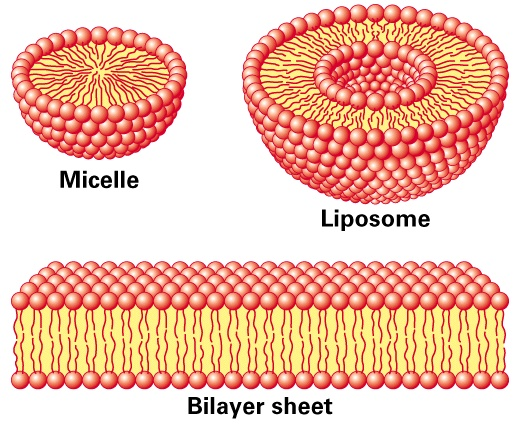
\includegraphics{Images/FattyAcidsInWater.JPG}
\caption{hydrophobicEffect}
\end{figure}

\end{document}
